\chapter{Informing student choice}\label{chap:5}

More and better information about university study will not help all prospective students decide on their tertiary education options. Only direct experience will persuade some that university is the right or the wrong place for them. But with so many prospective students uncertain about their direction, better advice should be available to them. One-in-five people who dropped out say they would not have enrolled if they had more information before they started.

Students should be alerted to the factors that increase the risk of completing. Prospective students planning to study part-time should be particularly warned. These factors should be included on websites that provide information to students, such as the Good Universities Guide and the Department of Education and Training's QILT (Quality Indicators for Learning and Teaching) website. The QILT site should be upgraded to enable students to enter their personal characteristics, so they can understand how risk factors interact. The site should also explain how students can mitigate the risks of non-completion.

\section{Clear and simple advice to prospective university students}\label{sec:5.1}

Many factors can affect whether students complete their degrees. But some factors are so significant that school advisers, university staff, and parents should alert prospective students to the risks in simple and general terms.

Young people should be encouraged to think first about whether university or vocational education would best suit them. As \Cref{sec:1.1} reported, university is now the default post-school activity for many young people. In their late-teenage years, two-thirds of young people plan to go to university.\footcite[][16]{MissionAustralia2016} 
These high aspirations are out of kilter with what is required to successfully complete a degree and the labour market's need for people with university qualifications.\footnote{See \textcite{Norton2017c} on graduate labour market outcomes.} Higher education demand has moderated in recent years, which is likely to be a sensible reaction to these trends. The fact that graduates do better in the labour market than non-graduates on average is not particularly useful information for prospective students at high risk of not obtaining professional or managerial employment.

For high-ATAR students, university clearly remains a good option. But those with lower ATARs are less likely to complete (\Cref{subsec:3.1.1}). Gender matters to the choices of lower-ATAR school leavers. Even with identical ATARs, men are less likely to complete university than women.\footnote{For more detail on the interaction between gender and ATAR, see the background paper, \textcite[][sections~3.1 and 5.1]{Cherastidtham2018a}.} On the other hand, men are much more likely than women to gain a financial benefit from vocational education (\Cref{subsec:2.1.3}).

These factors both suggest we should encourage young men with lower ATARs to think seriously about a vocational diploma or a Certificate III/IV qualification. Although mature-age study creates additional risks, vocational qualifications do not preclude university later in life. As \Cref{subsec:3.1.1} reported, students entering university with a prior vocational diploma qualification have reasonably good completion prospects, typically better than those without such qualifications but with otherwise similar backgrounds.

Young people choosing university should be encouraged to go as soon as possible after leaving school, to study full-time and to enrol on-campus. Delaying university only adds slightly to the risk of not completing, if it is just one year to age 19 (\Cref{subsec:3.1.5}). But delays increase the chance of distractions such as work once studies commence. Those who are older when they start studying are more likely to work full-time.\footnote{See \textcite[][section~5.4]{Cherastidtham2018a}.} 
People who work full-time before beginning their degree can get used to earning more, making them reluctant to forgo that income as a student. But no potentially avoidable factor is more harmful to completion prospects than studying part-time while juggling multiple commitments (\Cref{subsec:3.1.2}).

After controlling for all other factors, off-campus study adds only slightly to the risk of non-completion (\Cref{subsec:3.1.3}). For full-time students who genuinely can't get to a campus, off-campus study is better than not attending. But for students who can commute or move, studying on-campus should slightly increase their completion prospects, and add to the non-academic benefits of studying. As \Cref{subsec:2.1.3} reported, lasting friendships and connections are often a positive outcome of attending university.\footnote{Some other private benefits of higher education, including health, and some public benefits, including volunteering and civic attitudes, are plausibly linked to social networks at university: see \textcite{Savage2012}.}

Prospective mature-age students are the most complex case for general advice. Compared to starting university straight after school, commencing at an older age in itself adds up to 8 percentage points to the risk of non-completion (\Cref{subsec:3.1.5}). Mature-age students are much more likely than school leavers to study part-time, and to have other risk attributes such as studying online or being from an equity group. Because high-ATAR students usually begin their studies straight after school, mature-age students tend to have lower ATARs (\Vref{fig:1}). Such students are more likely to complete university if they have completed other post-school qualifications, which prepare them for academic study.

For mature-age students, advice to study full-time and on-campus may simply be impractical. It may be too difficult for them to change their other commitments. But some mature-age students do make the transition from part-time to full-time study. By their second year, about a third of the remaining mature-age students who began part-time have converted to full-time study.\footnote{\textcite[][]{DepartmentofEducationandTraininga}. `Mature age' defined as aged 25 or more on commencement.} Their completion rate is much higher than those who continuously study part-time (\Cref{subsec:3.1.2}). If at least periods of full-time study are possible, mature-age students should seriously consider it. For students who cannot study full-time at all, any advice is partly a warning: the vast majority of people who study only part-time won't get a degree in the next eight years.

\section{Integrate information about completion rates into QILT}\label{sec:5.2}

Some people could improve their higher education choices if information was more easily available. In the Grattan survey of people who had dropped out of a course, about one-in-five said they would not have enrolled had they had more information before they started. A slightly larger group were unsure (the other half would have started anyway, reflecting the benefits of an incomplete degree described in \Chapref{chap:2}).

Some prospective university students already use information about completion prospects. Applications, acceptances and enrolment data all show that lower-ATAR students exercise greater caution than high-ATAR students, and progressively larger numbers decide against university.\footnote{\Cref{sec:1.1} and \textcite[][tables~A8.1 and A8.2]{DepartmentofEducationandTraining2017b}.}

ATAR's connection with completion is unsurprising. But the links between other factors and completion are less intuitive. Prospective students are therefore taking risks they may have avoided if they had been better informed. The most significant of these risks is part-time study. For mature-age students, part-time study might seem like a sensible and convenient way to deal with the competing demands of work and family. But for many of them it doesn't work out, and they leave university without completing their course (\Cref{subsec:3.1.2}).

Some students who drop out of university have found from their own experience what they could have learned from the experience of others: that they aren't academically ready for university, or that there are too few hours in the day to combine study, work and family. If they had known that they were in the group of people with a less-than-50 per cent chance of completing university in eight years, they may not have enrolled in the first place, or enrolled only after they found a better way to manage the competing demands on their time.

As in many other fields, in higher education a website is the easiest way to get information to a wide audience. Higher education has a commercial website, the Good Universities Guide, and the Department of Education and Training's QILT (Quality Indicators for Learning and Teaching) website. The Good Universities Guide includes information on school-leaver student retention into second year, giving universities ratings of up to five stars on this and other indicators. But it does not cover other types of student, does not give information on fields of education (which, as \Cref{subsec:3.1.3} shows, can vary significantly in their completion rates), and does not distinguish between enrolment types. For example, retention rates largely driven by full-time students are misleading for a prospective part-time student.


Prospective students using QILT choose fields and universities of interest, and the website then provides them with comparative information on student satisfaction and graduate outcomes. QILT has no data on student retention or completion, and this is not otherwise easily available from government sources, either to prospective students or the people advising them.\footnote{The best existing source of information on completion by personal characteristics and study method is a now-regular report from the \textcite{DepartmentofEducationandTraining2017}. The best existing source of information on retention into second year is in the Department's annual student statistics release:
\textcite[][appendix~4]{DepartmentofEducationandTraining2017a}. However, each is located in a difficult-to-find part of the Department's website.} Adding that data to QILT, both to alert students to potential risks and to help them choose between courses, would be helpful.

QILT's presentation of information by university and field should stay, to ensure consistent presentation. But as \Chapref{chap:3} shows, there are many individual characteristics and study choices that can make average results unreliable. For the QILT data to be more useful for prospective students, it needs to be more personalised.

Personalising data would require prospective students to provide information relevant to calculating their completion prospects. This would include basic personal characteristics, such as age and gender, and then academic history and proposed study approach -- full-time or part-time, on-campus or off-campus, now or delayed. If prospective students provided this information, when they looked at courses of interest they could see their completion prospects, based on the outcomes of similar students in the past.

\vspace{6cm} %6cm of vertical space
\pagebreak

For example, a hypothetical 25-year-old male student from a remote area planning to study full-time at his nearby regional university campus faces a non-completion risk of 36 per cent. This means nearly 4-in-10 students in his situation are not expected to complete. He is considering moving to the city to study, which would reduce his risk to 32 per cent. But moving to the city means he has to move out of his parents' home, pay rent, and get a job. So he is considering studying part-time and online to accommodate his work schedule. Dropping 4 subjects to part-time would increase his risk to 64 per cent and online would increase it marginally further to 66 per cent. This means nearly 7-in-10 students in his situation would not complete. So while moving to the city to study would reduce his risk moderately, if this meant he had to study part-time he is better off studying near home to avoid increasing his risk substantially. The website could show, as \Vref{fig:extra1} does, that part-time study alone would make him nearly twice as likely to not complete within eight years. 

                % Figure extra1
                \begin{figure}[t]
                    \caption{Studying full-time minimises the risk of not-completing university\label{fig:extra1}}%
                    \units{Risk of not completing university within eight years, per cent}
                    \includegraphics[page=40]{atlas/selection_chartdeck.pdf} 
                    \noteswithsource{This hypothetical prospective student is  assumed to be a non-Indigenous male Australian citizen who speaks English at home, reports no disability, lives in a median SES area of NSW, lives 20- to-40 minutes from campus, and starts university in the first semester. He uses a previous diploma as his basis of admission.}
                    {Grattan analysis of \textcite{DepartmentofEducationandTraininga}}
                \end{figure}

QILT should also advise prospective students on how to improve their completion prospects. For example, if a prospective student is considering part-time study, the website would explain the difficulties of managing multiple competing demands on a student's time. This would enable prospective students to make a better-informed decision as they weigh up their options. As discussed in \Cref{subsec:3.1.2}, substantial proportions of the part-time students who persist past first year will switch to full-time study. They may have discovered at cost that the QILT website could and should have told them for free before they enrolled: that studying part-time substantially increases their risk of dropping out of university.

